\documentclass[class=jsarticle, crop=false, dvipdfmx, fleqn]{standalone}
%% preamble for Numerical-structure-analysis report

\input{/Users/User/Documents/Project/TeX/preamble/mypreamble}

%% titles
\title{先端データ解析論 レポート}
\author{37-196360 \quad 森田涼介}


%% setting for listings
\newtcbinputlisting[auto counter]{\reportlisting}[3][]{%
	listing file = {#3},
	listing options = {language=python, style=tcblatex, numbers=left, numberstyle=\tiny},
	listing only,
	breakable,
	toprule at break = 0mm,
	bottomrule at break = 0mm,
	left = 6mm,
	sharp corners,
	drop shadow,
	title = Listings \thetcbcounter : \texttt{#2},
	label = #1,
	}



%% title format
\usepackage{titlesec}
\titleformat{\section}{\LARGE}{宿題\thesection}{0zw}{}
\newcommand{\sectionbreak}{\clearpage}
\titleformat{\subsection}{\Large}{\Alph{subsection})}{0zw}{}

\begin{document}
\section{}

\begin{equation}
    T(z) = \lambda |z| + u (\theta - z) + \frac{1}{2} (\theta - z) ^2
    \qquad (\lambda \ge 0)
\end{equation}
について,
\begin{equation}
    \arg\min_z T(z) = \max(0,\ \theta + u - \lambda) + \min(0,\ \theta + u + \lambda)
\end{equation}
であることを証明する。

\begin{align}
    \pdv{T}{z}
        & = \lambda \mathrm{sign}(z) - u + (z - \theta) \\
        & = z - (\theta + u - \lambda \mathrm{sign}(z)) \\
    \pdv[2]{T}{z} & = 1 \quad (> 0)
\end{align}
より,\(T\)は下に凸な関数である。
以下では\(z\)の正負について場合分けをし,
\(T\)に最小を与える\(z\)を求める。

\(z \ge 0\)のとき,
\begin{equation}
    \pdv{T}{z} = z - (\theta + u - \lambda)
\end{equation}
\begin{enumerate}
    \item \(\theta + u \le \lambda\)のとき \\
        \(\forall z \ge 0\)に対して\(\pdv*{T}{z} \ge 0\)が成立し,\(T\)は増加関数となるので,
        \(T\)に最小を与える\(z = 0\)となる。
    \item \(\theta + u \ge \lambda\)のとき \\
        \(T\)は下に凸な関数であるから,\(\pdv*{T}{z} = 0\)を与える\(z\)が\(T\)に最小を与える。
        よって\(z = \theta + u - \lambda\)となる。
\end{enumerate}
これをまとめると,
\begin{equation}
    \arg\min_z T(z) = \max(0,\ \theta + u - \lambda)
\end{equation}

\(z \le 0\)のとき,
\begin{equation}
    \pdv{T}{z} = z - (\theta + u + \lambda)
\end{equation}
\begin{enumerate}
    \item \(\theta + u \ge -\lambda\)のとき \\
        \(\forall z \le 0\)に対して\(\pdv*{T}{z} \le 0\)が成立し,\(T\)は減少関数となるので,
        \(T\)に最小を与える\(z = 0\)となる。
    \item \(\theta + u \le -\lambda\)のとき \\
        \(\pdv*{T}{z} = 0\)を与える\(z = \theta + u + \lambda\)が\(T\)に最小を与える。
\end{enumerate}
これをまとめると,
\begin{equation}
    \arg\min_z T(z) = \min(0,\ \theta + u + \lambda)
\end{equation}

以上をグラフで表すと,図\ref{fig:z_theta_curve}のようになる。

\begin{figure}
    \centering
    \documentclass[class=jsarticle, crop=false, dvipdfmx, fleqn]{standalone}
%% preamble for Numerical-structure-analysis report

\input{/Users/User/Documents/Project/TeX/preamble/mypreamble}

%% titles
\title{先端データ解析論 レポート}
\author{37-196360 \quad 森田涼介}


%% setting for listings
\newtcbinputlisting[auto counter]{\reportlisting}[3][]{%
	listing file = {#3},
	listing options = {language=python, style=tcblatex, numbers=left, numberstyle=\tiny},
	listing only,
	breakable,
	toprule at break = 0mm,
	bottomrule at break = 0mm,
	left = 6mm,
	sharp corners,
	drop shadow,
	title = Listings \thetcbcounter : \texttt{#2},
	label = #1,
	}



%% title format
\usepackage{titlesec}
\titleformat{\section}{\LARGE}{宿題\thesection}{0zw}{}
\newcommand{\sectionbreak}{\clearpage}
\titleformat{\subsection}{\Large}{\Alph{subsection})}{0zw}{}

\begin{document}
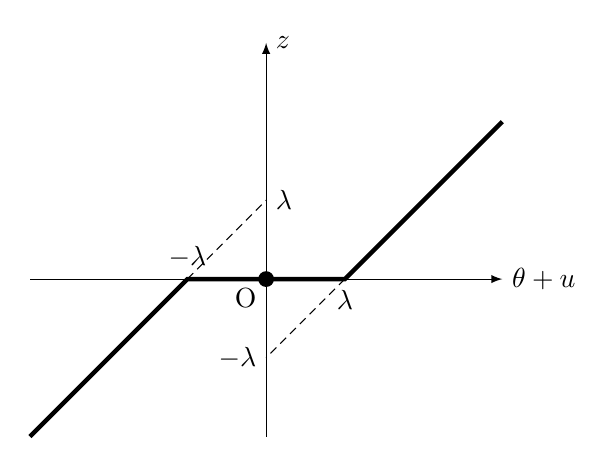
\begin{tikzpicture}

% coordinates
\coordinate (O) at (0, 0);
\fill (O) node[below left]{O} circle [radius=1mm];


% axis
\begin{scope}
    \draw [-latex] (O)--+(3, 0)node[right]{\(\theta + u\)};
    \draw (O)--+(-3, 0);
    \draw [-latex] (O)--+(0, 3)node[right]{\(z\)};
    \draw (O)--+(0, -2);
\end{scope}


% graph
\begin{scope}[ultra thick]
    \draw (O)
        to (1, 0) node[below]{\(\lambda\)}
        to (3, 2);
    \draw (O)
        to (-1, 0) node[above]{\(-\lambda\)}
        to (-3, -2);
\end{scope}

\begin{scope}[densely dashed]
    \draw (1, 0) to (0, -1) node[left]{\(-\lambda\)};
    \draw (-1, 0) to (0, 1) node[right]{\(\lambda\)};
\end{scope}
\node [above right] at (0, 0) {};



\end{tikzpicture}
\end{document}

    \caption{\(z - \theta+u\)曲線}
    \label{fig:z_theta_curve}
\end{figure}

以上より,
\begin{equation}
    \arg\min_z T(z) = \max(0,\ \theta + u - \lambda) + \min(0,\ \theta + u + \lambda)
\end{equation}
であることがわかる。


\end{document}
